The $\mathbb{R}^k$ range searching for minimum algorithm works as follows. Dimensions $k,k-1 \ldots 2$ are scaled. The data structure for dimension $k (k \geq 2)$ is a scaling tree, where each node has a data structure for $\mathbb{R}^{k-1}$ range searching for minimum. In dimension 2, each node has a list of its points sorted on $x_j$ value, with line pointers to the lists of its children.\\

\begin{figure}[H]%
    \centering
    \subfloat[Cartesian tree for 1D \emph{RMQ}]{{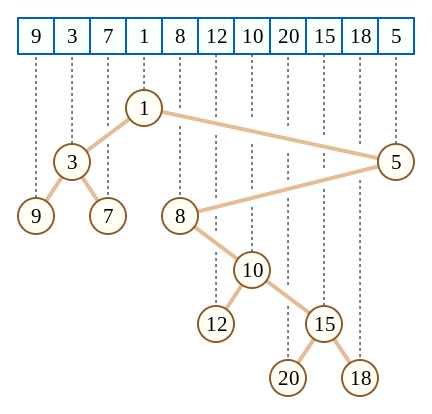
\includegraphics[width=6cm,height=4cm]{img/Cartesian_tree.png} }}%
    \qquad
    \subfloat[Solving 2D \emph{RMQ}]{{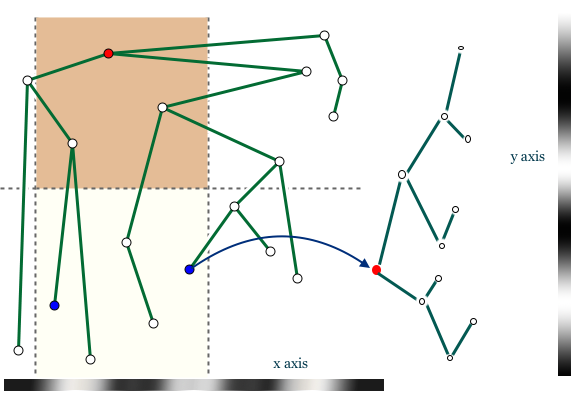
\includegraphics[width=8cm,height=4cm]{img/2D_Cartesian_tree.png} }\label{fig:2d_cartesian}}%
    \caption{Solving \emph{RMQ} with cartesian tree \cite{wiki:xxx}}%
    %\label{fig:example}%
\end{figure}

Later in 2003 Poon presented a new data structure to support orthogonal range max queries on datacube \cite{p6}. Since orthogonal datasets can be considered as a $n$-dimensional array, the range max queries can be considered same as \emph{RMQ} queries. OLAP databases frequently uses aggregate queries and fast response time is essential for it. Poon came up with a data structure that has $\mathcal{O}(c^d_1)$ query time and $\mathcal{O}((c_2n)^d)$ storage for $d < c_3 \log \log n / \log(\log^* n)$ and some constants $c_1$, $c_2$ and $c_3$ independent of $d$ and $n$. So for a fixed dimension the query time is constant.  \\

\begin{figure}[H]%
    \centering
    {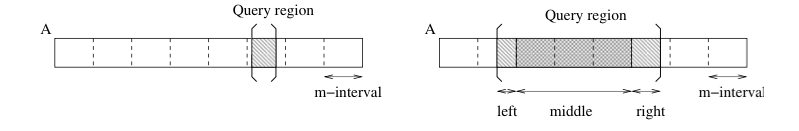
\includegraphics[width=14cm,]{img/poon.png} }
    \caption{Solving 1D \emph{RMQ} with Poon micro and macro structure \cite{p6}}%
    \label{fig:poon1d}%
\end{figure}


This paper introduced the concept of the macro and micro-structures and similar structure has been used for RAM implementation in this paper. The macro-structure $X$ is an array of $\mathcal{O}(n)$ constructed as a range max structure on $A_m$; where main array is divided into $m$ blocks and $A_m[i]$ consists of min or max of $i^{th}$ block. $X$ takes $\mathcal{O}(n)$ construction time. The micro-structure consists of an array $Y$ of length $n$. Each array position $i$ in $A$ will be associated with the word $Y[i]$. It stores only the index to the answer for each place in the block which is between $0$ to $m-1$. Hence it requires $m \log m$ bits for $Y[i]$. This is feasible since $m \log m$ = $(c \log^* n)\log(c \log^* n)$ $\leq$ $b \log n$ for sufficiently large $n$.

To answer a query [$ i \ldots j]$ consider figure \ref{fig:poon1d} with two cases. Firstly, when the query range is within a block we make use of micro structure to compute answer. Secondly, when the query range spans across two or more $m$-intervals or blocks, the leftmost and rightmost part can be answered by micro structure which takes 2 steps each. The middle intervals are calculated by macro structure $X$ with 4 steps. Hence it requires at most 8 steps.

In 2D, for each $i \in [0..n - 1]$, it constructs a macro-structure for $A[i][0..n - 1]$. Let them be stored in an array $B[0..n - 1][0..n - 1]$. Then for each $j \in [0..n - 1]$, it constructs a 1-dimensional range max/min structure (including both macro- and micro-structures) for $B[0..n - 1][j]$. Let the resultant structures be stored in $X[0..2n - 1][0..n - 1]$.

Next, it constructs a macro-structure for $A[0..n - 1][j]$ for each $j \in [0..n - 1]$ and stores in $C[0..n-1][0..n-1]$. Then a micro-structure for $C[i][0..n-1]$ for each $i \in [0..n-1]$ is constructed. Let them be stored in $Y [0..n-1][0..n-1]$.\\
Finally, a 2-dimensional micro-structure $Z[0..n-1][0..n-1]$ is computed such that $Z[i][j]$ stores the $m^2$ answers to the $m^2$ query regions: $[i..i + x] \times [j..j + y]$ where $0 \leq x,y < m$. Again, the offsets of the position of the answer from $i$ and $j$ are stored respectively. Thus, each 2-dimensional offset requires $2 \log m$ bits. This is feasible as long as $m^2 \log(m^2) \leq b \log n$.\\
In total, it needs to store the arrays, $A,B,C,X,Y$ and $Z$, using a total of $7n^2$ storage. The construction time is therefore $\mathcal{O}(n^2m + (n/m)^2m^4) = \mathcal{O}((nm)^2)$.

\begin{figure}[H]%
    \centering
    \subfloat[]{{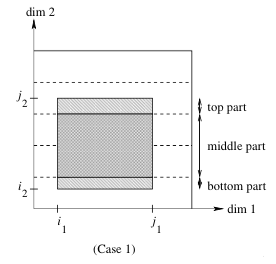
\includegraphics[width=5cm,height=5cm]{img/2dpoon1.png} }\label{fig:2d_poon1}}%
    \qquad
    \subfloat[]{{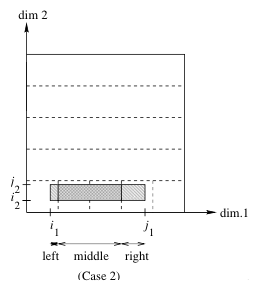
\includegraphics[width=5cm,height=5cm]{img/2dpoon2.png} }\label{fig:2d_poon2}}%
    \qquad
    \subfloat[]{{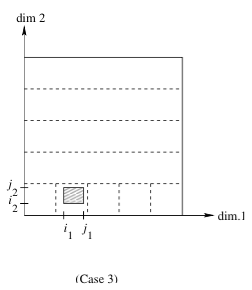
\includegraphics[width=5cm,height=5cm]{img/2dpoon3.png} }\label{fig:2d_poon3}}%
    \caption{Solving 2D \emph{RMQ} with Poon's approach \cite{p6}}%
    %\label{fig:example}%
\end{figure}

To answer queries in 2D three cases are considered. Case $1$, query spans more than one $m$-intervals in dimension $2$, in which the middle part can be answered in 32 steps with the help of macro-structure $A$ and $X$. The top and bottom part are covered in case $2$ and $3$. In case $2$, the query lies within one $m$-inteval of dimension $2$ but spans across more than one $m$-interval in dimension $1$. This requires macro structure $A$, $C$ and micro structure $Y$ to answer in 8 steps. Case $3$, the query lies with in both one $m$-interval in both dimension, where it requires lookup in micro structure $Z$ with proper offset and a lookup in $A$. This takes 56 steps. (Detailed theoretical analysis is found in paper \cite{p6})

For $d$-dimension, Poon gave a theoretical bound as $8^d$ as the number of steps required in worst case to answer $d$-dimension \emph{RMQ} which requires $\mathcal{O}(3^d)$ storage space and $\mathcal{O}((3nm)^d)$ preprocessing time. Here we can conclude that Poon's contribution is a milestone in \emph{RMQ} field. Later Amir et al. \cite{p7} showed that preprocessing time can be reduced to a significant extent. However his work is not for general $d$-dimension but his approach is worth considering.


Amir et al. solved 2D \emph{RMQ} with $\mathcal{O}(kN)$ additional space, preprocessing time of $\mathcal{O}(N \log^{[k+1]}N$ to answer queries in constant time for any $k>1$. The ability to trade off between storage space and preprocessing time is a significant development. The idea of the preprocessing algorithm is to cover the input array with grid or intervals of decreasing width $s_1, s_2,s_3,\ldots$ thus dividing the array into block of decreasing size. For each grid $s_i$ it preprocesses the array such that any queries which cross grid of $s_i$ but do not cross grid $s_{i'}$; where $i' < i$, can be queried in constant time. 


\begin{figure}[H]%
    \centering
    \subfloat[]{{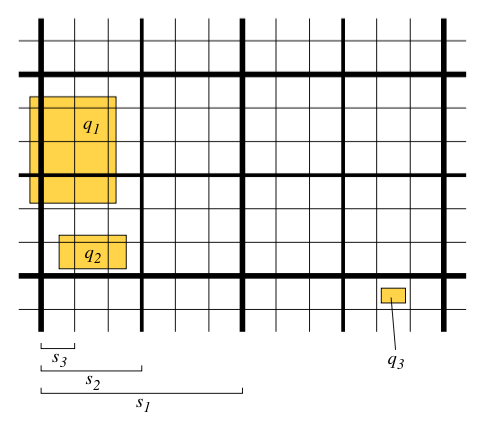
\includegraphics[height=4cm]{img/amir1.png} }\label{fig:amir1}}%
    \qquad
    \subfloat[]{{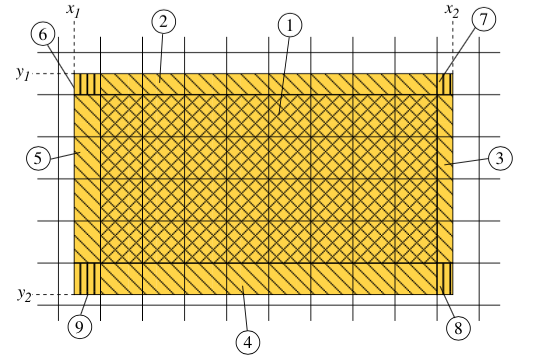
\includegraphics[height=4cm]{img/amir2.png} }\label{fig:amir2}}%
    \caption{Grid structure proposed by Amir et al. \cite{p7} }%
    %\label{fig:example1}%
\end{figure}


In Fig. \ref{fig:amir1}, $q_1$ will be answered at level 1 since it crosses grid of width $s_1$ and $q_2$ will be answered in level 3. For query with in a grid i.e. does not cross any grid, will be answered from a precalculated all queries from microblocks. If size of microblocks is constant, no extra preprocessing time is required and will lead to $\log^*$ solution, else a sorting of block is needed for constant time preprocessing which leads to $\mathcal{O}(N \log^{[k+1]} N)$ preprocessing time.

Fig \ref{fig:amir2} decomposes a query into 9 subqueries. Query 1 is answered by calculating minimum of 4 equal sized overlapped rectangles whose side lengths are power of 2. Query 2-5 are similar where query spreads over several grids but not sharing superblock grid and it takes at most 2 internal queries. The significant part of this analysis is the amount of storage space required is $\mathcal{O}(N)$. For Query 6-9 the blocks of sizes $2^1, 2^2, 2^3,\ldots$ are already precomputed and \emph{RMQ} is answered form those grid blocks. (Here we don't have enough scope for detailed analysis, refer \cite{p7} for more). 

Amir, Fischer, and Lewenstein conjectured that in two dimensions there is no such nice relation as the one between the number of different \emph{RMQ}s and the number of different Cartesian Trees in one dimensional case. Demaine, Landau and Weimann \cite{p2} proved this conjecture to be true i.e. no Cartesian tree exists for the two-dimensional version of the range minimum query problem. It is worth mentioning here Atallah, Yuan's noble approach caught attention very early and Demaine et al. \cite{p2} mentioned its manuscript.

\section{Notational Preliminaries}
Let's define $A$ as the input array of $d$-dimensions. We assume the length of each dimension denoted by $n_k$ for $1\leq k\leq d$ to be power of $2$. This assumption simplifies the explanation of the algorithms without any loss of generality. And it also would not change any complexity bounds derived. The indices for $k^{th}$ dimension is denoted by $[1,n_k]$. For a $d$-dimensional range $q=[a_1,b_1]\times[a_2,b_2]\times\ldots\times[a_d,b_d]$, $A[q]$ is defined to be the subarray induced by $q$. Now $RMQ(A,q)=\min A[q]$, i.e. the minimum element in the subarray $A[q]$. The indices for $k^{th}$ dimension a subarray are assumed to be $[1,b_k-a_k+1]$. The array entries are assumed to be distinct without any loss of generality, so that for any range there is only $1$ minimum element. But this can be enforced by breaking ties by introducing some consistent ordering (like lexicographic ordering).$POS(A,q)$ is a $d$-dimensional vector denoting index of $RMQ(A,q)$. The size of a range is defined as the number of integer coordinates that are contained in the range and is denoted by $\left\vert q\right\vert$. For example the range $q$ mentioned in the beginning has $(b_1-a_1+1)\times(b_2-a_2+1)\times\ldots\times(b_d-a_d+1)$ elements in it where $a_i,b_i$ are all integers. Therefore, if $\left\vert q\right\vert =1$, then $A[q]$ denotes a particular entry instead of a subarray. No assumptions have been made on the element type of the array $A$, the only assumption is that they are comparable.




